\documentclass[final,a4paper,12pt]{article}

\usepackage[margin=1in]{geometry}

\usepackage{color}
\usepackage{listings}
\lstset{ %
language=C,            	    	% choose the language of the code
basicstyle=\footnotesize,       % the size of the fonts that are used for the code
numbers=left,                   % where to put the line-numbers
numberstyle=\footnotesize,      % the size of the fonts that are used for the line-numbers
stepnumber=1,                   % the step between two line-numbers. If it is 1 each line will be numbered
numbersep=5pt,                  % how far the line-numbers are from the code
backgroundcolor=\color{white},  % choose the background color. You must add \usepackage{color}
showspaces=false,               % show spaces adding particular underscores
showstringspaces=false,         % underline spaces within strings
showtabs=false,                 % show tabs within strings adding particular underscores
frame=single,           			% adds a frame around the code
tabsize=2,          				% sets default tabsize to 2 spaces
captionpos=b,           			% sets the caption-position to bottom
breaklines=true,        			% sets automatic line breaking
breakatwhitespace=false,    		% sets if automatic breaks should only happen at whitespace
escapeinside={\%*}{*)}          % if you want to add a comment within your code
}

\usepackage{graphicx}
\graphicspath{{figures/}}

\author{Floris den Heijer\thanks{Dr. Clemens Grelck}\\
 FNWI, University of Amsterdam\\
 floris@denheijer.com}
 
\date{\today}

\title{A Modern Civic Compiler Framework}

\setcounter{tocdepth}{3}
\setcounter{secnumdepth}{3}

\begin{document}

\maketitle
\clearpage

\tableofcontents
\clearpage

\section*{Language selection}
Realistically the choice is one of C, C\#, Java, F\# or Scala, though functional languages are not prefered.

Considering a large portion of the project (so far) is spend on prototyping, the author's familiarity with C\# and the fact that C\# is syntactically similar to Java, the rest of the draft will feature this language. It must be noted that C\# supports constructs such as lambda expressions and co- and contra-varianct interfaces, which Java does not.

This is a draft, this section will be supplemented with proper arguments. 

\section*{Other topics}
\begin{itemize}
	\item AST vs ASG
	\begin{itemize}
		\item Traversals annotate and augment AST to create some form of graph
		\item Current framework explicitly states which nodes are to be traversed as `sons', this means not all properties of a class of type `Node' are to be traversed
	\end{itemize}
	\item Is an AST more than a parse tree validator? 
	\item Related patterns: Composite, Visitor, MultiMethod, Hierarchical Visitor Pattern, Graph traversals
	\item Continuation Passing Style
	\item Paper: On understanding types, data abstraction, and polymorphism (1985)
	\item It would be nice to have an aggregate visitor or a traversal which can be invoked on a (sub-)tree.
	\begin{itemize}
		\item Following the Command Query Seperation principle, this traversal should not modify the graph
	\end{itemize}
\end{itemize}
\clearpage

\section*{Composite and visitor design pattern}



\section{Analysis of the current framework}
Short introduction on the framework, functionality outline, boundaries, etc. It makes sense to begin with a review of the AST.
\begin{itemize}
	\item Structured source code transformation with phases
	\item Abstract syntax tree defined seperate from code
	\item Code generator for AST nodes, traversals, validation phase
	\item Debug helpers
	\item Documentation generator for AST
	\item Wrappers for common C functionality and extensions
\end{itemize}

\subsection{Abstract syntax tree}
The abstract syntax tree - or AST - is the heart of the framework. It defines the relation between nodes and is able to validate a tree and possibly prohibit invalid operations. It is defined in an XML file, which is parsed on compilation by a code generator. This generator in turn creates C code for the node structures, property accessors, construction helpers, traversals and validation mechanisms.

The generated node struct is a tagged union, which uses a tag field to identify the type of the node. C does not provide compiler guarantees on tagged unions, though limited type safety can be enforced by strictly controlling access to node instances [ref]. The  framework does this by generating property accessor typedefs which are the only way to modify or access node attributes. In these typedefs debug assertions are placed which guarantee the attribute accessed belongs to the node.

Additional insurance is provided by the traversal function, which only invokes traversal handlers if the node type matches. [does it guarantee this?] [Todo: can user code set the node type? If not, who can?]

An AST node may require it's children to be of a specific set, for instance a `while-loop' has a child `condition' which is an expression. An expression could be a variable reference, function call or ternary, but not a statement. This construct is supported by introducing `node sets' in the AST, which are a list of node types. Node declarations may reference these sets within the AST to constrain attributes. [Todo: are node sets also checked when updating a child variable? Is there logic in the typedef or in the validation phase?]

The AST definition is more than just a specification, as it is responsible for the correct translation of:
\begin{itemize}
	\item Node types for the code generator, as well as the C types of attributes
	\item Traversal phases and targets
	\item Additional attribute validation
\end{itemize}

\subsection{Traversals}
\subsection{Error handling}
\subsection{Strength weakness analysis?}
Strength-weakness analysis without mud throwing and without AST, as this is handled below.

This analysis demonstrated that reasonable checks are in place to prevent basic type mix-ups. While this layer of protection is enough for experienced framework programmers, it is in no way a replacement for a modern type system.


\section{Moving to a managed language}
One of the objectives of this project is to investigate how we might implement an the framework in language which supports classes, polymorphism and better compile time type safety. The lack of a type system is likely one of the reasons for the seperation of specification and declaration, as guaranteeing strict access to union structs is tedious and easily done wrong.

When stripped of its type safety mechanisms the framework looks very different.

The strict access control to node attributes is handled by compiled time type safety, which raises the question if there is any benefit in seperating specification from code. A hand written AST definition is arguably more error prone than code, as code has the benefit of compile time checks which XML does not.

The node sets could probably be replaced in its entirity with class inheritance. User defined functions are no longer necessarily global, but are instead compartmentized in namespaces. Wrappers for C system functions are replaced with a managed framework, offering better documentation and greater ease of use.

In a language with type safety the framework - as is - does not make much sense.

\subsection{Repositioning the AST}
An interesting thought is to position the AST firmly in the user domain. In light of the old framework this is freedom of preposterous proportions. Is this always a good thing?

When defining an AST in pure code, it is important to maintain a clear picture of what is reasonable and what is not. If the subject matter is not known it's not very difficult to invent esoteric solutions to problems which never would have existed before.

One way to regain territory is by compensating in other areas. If the built-in visitors do not support the AST, most likely a student would change his code. But then again, in a decoupled system he or she could also replace whatever functionality is not wanted and soldier on. In a way this hypothetical scenario accomplishes what the original framework couldn't do: promote interaction with the underlying system. The only trouble is that so far we don't have anything resembling a framework yet.

\subsection{Design considerations}
In this section the influence of the structure of an AST with regards to user- and framework interation is examined. What is the best way to handle collections and how does this effect traversal? Can we identify all reasonable implementations for a code based AST and how does any of this effect type safety?

\subsubsection{Representing collections}
Collections are used to represent a node which has a variable number of child nodes. There are at least two ways to represent such a collection in a tree:
\begin{enumerate}
	\item Linked lists embodied in the tree structure (figure~\ref{fig:sll} and~\ref{fig:dll})
	\item List or dynamic array as an attribute of a node (figure~\ref{fig:list})
\end{enumerate}

\begin{figure}[ht]
	\begin{minipage}[b]{0.45\linewidth}
		\centering
		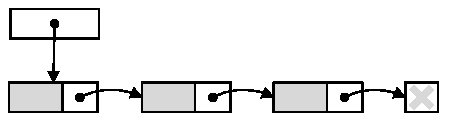
\includegraphics[width=\textwidth]{sll}
		\caption{Singly linked list}
		\label{fig:sll}
	\end{minipage}
	\hspace{0.5cm}
	\begin{minipage}[b]{0.45\linewidth}
		\centering
		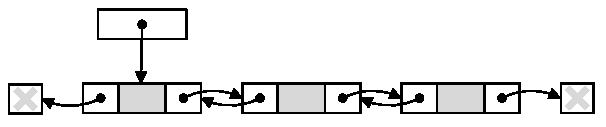
\includegraphics[width=\textwidth]{dll}
		\caption{Doubly linked list}
		\label{fig:dll}
	\end{minipage}
\end{figure}
\begin{figure}[h]
	\centering
	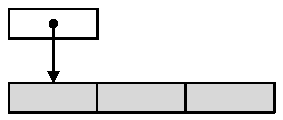
\includegraphics{list}
	\caption{Dynamic array or list structure}
	\label{fig:list}
\end{figure}

Child nodes (shown in grey) are in held in a wrapper object responsible for pointers to other wrappers in the case of a linked list, or the maintaince of the list itself. While both constructs are similar in that expose an ordered set of child nodes, they are not interchangeable.

Wrappers for linked lists can be implemented as nodes with navigational properties, 

Additionally 

\section*{Deep copy}
The original Civic framework uses code generation to produce a traversal which copies (a portion of) a tree. In C\# this requires a deep copy of the root object, which is not supported by default. There are several ways to create a deep copy:

\begin{enumerate}
	\item Add clone() method to base class; each node must implement this call (fragile, manual labour)
	\item Serialize object, then deserialize (might skip private fields)
	\item Use reflection recursively, extend object (incomprehensible)
\end{enumerate}

It just so happens the last method is the most effective, and supported by a library (under MIT license). Source code is available. It would be foolish to implement this manually, mistakes are easy to make and it would clutter the framework with more reflection code.

\section*{Phase validation}
An AST can be invalid in a number of ways [also, is the AST the template, or definition? or the parsed tree?] For instance, it might contain a node of a wrong type in a certain position. These errors are mostly eliminated with subclassing. Another type of invalidity might come from the lack of a node in a position.

Variables of an object type in languages like C\#, C++ or Java may have a null value; null can be assigned in any position where one might expect an instance of such an object.

Ideally we would like to perform certain validations at certain points in the transformation of the AST. When using backlinks created in an earlier phase it would be useful for future phases to skip assertions on these links.

Dynamically determined, validation traversal? Bound to phase or order of phase. Postcondition.

Only useful for debugging? Null reference isn't too bad during development.. Concrete examples needed. Simple solution would be to invoke `AddBacklinks' traversal before (or during) phase which requires it.

Or perhaps a custom validation traversal, inserted as needed? This determines the `shape' of the AST.

\subsection*{Code contracts in C\#}
Precondition, postcondition, invariant, result.

\subsection*{Scaling}
How does any approach scale to larger compilers? What internal structures do they use? (AST transformation through phases, seperate AST for each phase).

\section*{Variable initialization scope}
Needs to be clarified, two different styles methods exist: needs clarification.

\begin{lstlisting}[caption=Ambiguity in variable references]
int x = 1;

void proc() {
	//	x from global scope or self reference?
	int x = x;

	void proc() {
		//	also for local funcs
		int x = x;
	}

	for (int x = x, x, x) {
		//	.. and iterators
	}
}
\end{lstlisting}

\section*{Error handling}
asdf

\end{document}




















































